% !TEX program = xelatex
\documentclass[a4paper,10pt]{article}
\usepackage[UTF8,fontset=none]{ctex}
\usepackage{xeCJK}
\setCJKmainfont{Songti SC}
\setCJKsansfont{STHeiti}
\setCJKmonofont{Songti SC}
\usepackage[margin=2.2cm]{geometry}
\usepackage{tikz}
\usetikzlibrary{shapes.geometric, arrows.meta, positioning, calc, fit}
\usepackage{amsmath, amssymb}
\usepackage{longtable}
\usepackage{array}
\usepackage{booktabs}
\usepackage{multirow}
\usepackage{enumitem}
\usepackage{fancyhdr}
\usepackage{titlesec}
\usepackage{hyperref}
\usepackage{xcolor}
\usepackage{tabularx}

\hypersetup{
  colorlinks=true,
  linkcolor=blue!60!black,
  urlcolor=blue!60!black,
  bookmarksnumbered=true
}

% 页眉页脚
\pagestyle{fancy}
\fancyhf{}
\fancyhead[L]{\small fitWaypointTrajectory~函数设计文档}
\fancyhead[R]{\small 内部公开}
\fancyfoot[C]{\thepage}
\renewcommand{\headrulewidth}{0.4pt}

% 层级编号
\setcounter{secnumdepth}{3}
\setcounter{tocdepth}{3}

% 表格列宽辅助
\newcolumntype{L}[1]{>{\raggedright\arraybackslash}p{#1}}
\newcolumntype{C}[1]{>{\centering\arraybackslash}p{#1}}

% ============================================================
\begin{document}

% ==================== 封面表格 ====================
\thispagestyle{empty}

\begin{center}
{\CJKfamily{zhsong}\bfseries\Large 函数设计文档}
\end{center}

\vspace{8pt}

\begin{center}
\renewcommand{\arraystretch}{1.5}
\begin{tabular}{|L{3.2cm}|L{4.5cm}|L{3.2cm}|L{4.5cm}|}
\hline
\textbf{函数英文名} & fitWaypointTrajectory &
\textbf{函数中文名} & 路点轨迹拟合 \\
\hline
\textbf{函数类型} & 组件 (Component) &
\textbf{版本} & 2.0 \\
\hline
\textbf{作者} & 许庆 &
\textbf{日期} & 2026-06-26 \\
\hline
\textbf{联系方式} & \multicolumn{3}{l|}{18612426814~/~qingxu@tsinghua.edu.cn} \\
\hline
\textbf{密级} & 内部公开 &
\textbf{AI辅助} & Cursor Agent (Claude Opus 4.6) \\
\hline
\end{tabular}
\end{center}

\vspace{12pt}

\begin{center}
\renewcommand{\arraystretch}{1.4}
\begin{tabular}{|C{1.2cm}|C{2cm}|L{5cm}|C{2cm}|C{2cm}|}
\hline
\multicolumn{5}{|c|}{\textbf{更改记录}} \\
\hline
\textbf{版本} & \textbf{日期} & \textbf{更改说明} & \textbf{作者} & \textbf{AI辅助} \\
\hline
1.0 & 2026-06-20 & 初始版本 & 许庆 & --- \\
\hline
2.0 & 2026-06-26 & 重构：增加原点数据点、X归一化拟合、参考车速估算 & 许庆 & Cursor Agent \\
\hline
\end{tabular}
\end{center}

\newpage

% ==================== 目录 ====================
\tableofcontents
\newpage

% ============================================================
%  1. 函数需求
% ============================================================
\section{函数需求}

\subsection{功能概述}

\texttt{fitWaypointTrajectory} 将自车当前位置（原点 $(0,0)$）和 6 个参考路点共 7 个数据点
的 X 坐标归一化到 $[0,1]$ 后进行三次多项式最小二乘拟合，输出归一化轨迹多项式系数和参考车速。

包含原点的目的是确保 MPC 预测初始阶段的参考轨迹有效；X 归一化可避免大数值导致法方程条件数过大。

\subsection{输入/输出/返回值}

\renewcommand{\arraystretch}{1.3}
\begin{longtable}{|C{1.5cm}|L{3.5cm}|C{2.5cm}|L{7.5cm}|}
\hline
\textbf{方向} & \textbf{名称} & \textbf{类型} & \textbf{说明} \\
\hline
\endfirsthead
\hline
\textbf{方向} & \textbf{名称} & \textbf{类型} & \textbf{说明} \\
\hline
\endhead
输入 & \texttt{waypoints} & \texttt{const Waypoint*} & 路点数组（\texttt{NUM\_WAYPOINTS} 个），自车坐标系 \\
\hline
输入 & \texttt{numWaypoints} & \texttt{int} & 路点数量（典型值 6） \\
\hline
输入 & \texttt{egoSpeed} & \texttt{double} & 自车当前车速 (m/s) \\
\hline
返回值 & --- & \texttt{FittedTrajectory} & 拟合结果：多项式系数 \texttt{poly}、归一化参数 \texttt{xOffset}/\texttt{xScale}、参考车速 \texttt{refSpeed}、有效标志 \texttt{valid} \\
\hline
\end{longtable}

% ============================================================
%  1.2 算法设计
% ============================================================
\subsection{算法设计}

\subsubsection{数据准备}

将原点 $(0,0)$ 作为第 0 个数据点，与 $N$ 个路点合并，共 $N{+}1$ 个点：
\begin{equation}
  (x_0, y_0) = (0, 0), \quad (x_{i+1}, y_{i+1}) = (\text{waypoints}[i].x,\; \text{waypoints}[i].y), \quad i = 0,\ldots,N{-}1
\end{equation}

\subsubsection{X坐标归一化}

计算 X 坐标范围并归一化：
\begin{equation}
  x_{\min} = \min_i x_i, \quad x_{\max} = \max_i x_i, \quad \Delta x = x_{\max} - x_{\min}
\end{equation}
\begin{equation}
  \bar{x}_i = \frac{x_i - x_{\min}}{\Delta x}, \quad i = 0, 1, \ldots, N
\end{equation}

当 $\Delta x < 0.5$\,m 时，X 方向跨度过小，无法有效拟合，直接标记为无效。

\subsubsection{三次多项式拟合}

在归一化坐标系下进行三次多项式拟合：
\begin{equation}
  y(\bar{x}) = c_0 + c_1 \bar{x} + c_2 \bar{x}^2 + c_3 \bar{x}^3
\end{equation}

调用下级函数 \texttt{fitCubicPolynomial} 执行最小二乘拟合，内部构造 Vandermonde 法方程：
\begin{equation}
  (\mathbf{A}^{\!\top}\!\mathbf{A})\,\mathbf{c} = \mathbf{A}^{\!\top}\!\mathbf{y}
\end{equation}
其中 $\mathbf{A}$ 的第 $i$ 行为 $[1, \bar{x}_i, \bar{x}_i^2, \bar{x}_i^3]$。

\subsubsection{参考车速估算}

根据路点间累计弧长除以总时间跨度估算参考车速：
\begin{equation}
  d_0 = \sqrt{x_1^2 + y_1^2}, \quad
  d_i = \sqrt{(x_{i+1} - x_i)^2 + (y_{i+1} - y_i)^2}, \quad i = 1,\ldots,N{-}1
\end{equation}
\begin{equation}
  v_{\text{ref}} = \frac{\sum_{i=0}^{N-1} d_i}{T_{\text{total}}}, \quad T_{\text{total}} = 3.0\;\text{s}
\end{equation}

当拟合无效时，参考车速退化为当前自车车速 $v_{\text{ego}}$。

% ============================================================
%  1.3 程序流程图
% ============================================================
\subsection{程序流程图}

\begin{center}
\begin{tikzpicture}[
  node distance=0.9cm and 1.5cm,
  startstop/.style={rectangle, rounded corners, minimum width=3.5cm, minimum height=0.7cm,
    text centered, draw=black, fill=blue!8, font=\small},
  process/.style={rectangle, minimum width=5cm, minimum height=0.7cm,
    text centered, draw=black, fill=orange!8, font=\small},
  decision/.style={diamond, aspect=2.5, minimum width=2cm,
    text centered, draw=black, fill=green!8, font=\small},
  io/.style={trapezium, trapezium left angle=70, trapezium right angle=110,
    minimum width=3.5cm, minimum height=0.7cm,
    text centered, draw=black, fill=yellow!8, font=\small},
  arrow/.style={-{Stealth[length=2.5mm]}, thick}
]

\node (start) [startstop] {开始};
\node (input) [io, below=of start] {读入 waypoints, numWaypoints, egoSpeed};
\node (merge) [process, below=of input] {合并原点与路点, 共 $N{+}1$ 个点};
\node (range) [process, below=of merge] {计算 $x_{\min}$, $x_{\max}$, $\Delta x$};
\node (check) [decision, below=of range] {$\Delta x \geq 0.5$\,m?};
\node (invalid) [process, right=2.5cm of check] {标记 valid = false};
\node (norm) [process, below=of check] {X 坐标归一化 $\bar{x}_i$};
\node (fit) [process, below=of norm] {调用 fitCubicPolynomial};
\node (speed) [process, below=of fit] {计算路点间累计弧长};
\node (vref) [process, below=of speed] {$v_{\text{ref}} = \text{totalDist} / 3.0$};
\node (pack) [process, below=of vref] {组装 FittedTrajectory 结果};
\node (output) [io, below=of pack] {返回 FittedTrajectory};
\node (stop) [startstop, below=of output] {结束};

\draw [arrow] (start) -- (input);
\draw [arrow] (input) -- (merge);
\draw [arrow] (merge) -- (range);
\draw [arrow] (range) -- (check);
\draw [arrow] (check) -- node[above]{\small 否} (invalid);
\draw [arrow] (invalid) |- (pack);
\draw [arrow] (check) -- node[right]{\small 是} (norm);
\draw [arrow] (norm) -- (fit);
\draw [arrow] (fit) -- (speed);
\draw [arrow] (speed) -- (vref);
\draw [arrow] (vref) -- (pack);
\draw [arrow] (pack) -- (output);
\draw [arrow] (output) -- (stop);

\end{tikzpicture}
\end{center}

% ============================================================
%  1.4 函数接口 + 1.5 输入输出模块图
% ============================================================
\subsection{函数接口}

\begin{verbatim}
FittedTrajectory fitWaypointTrajectory(
    const Waypoint* waypoints,
    int numWaypoints,
    double egoSpeed);
\end{verbatim}

\subsection{输入输出模块图}

\begin{center}
\begin{tikzpicture}[
  box/.style={rectangle, draw=black, thick, minimum width=3.5cm, minimum height=0.7cm,
    text centered, fill=blue!6, font=\small},
  core/.style={rectangle, draw=black, very thick, minimum width=5.5cm, minimum height=2.0cm,
    text centered, fill=orange!10, font=\normalsize\bfseries, rounded corners=3pt},
  iobox/.style={rectangle, draw=black, thick, minimum width=3.2cm, minimum height=0.6cm,
    text centered, fill=yellow!10, font=\small},
  arrow/.style={-{Stealth[length=2.5mm]}, thick}
]

% 核心模块
\node (core) [core] {fitWaypointTrajectory};

% 输入 (左侧)
\node (in1) [iobox, left=3cm of core, yshift=0.8cm] {waypoints[6] (Waypoint)};
\node (in2) [iobox, left=3cm of core, yshift=0cm] {numWaypoints (int)};
\node (in3) [iobox, left=3cm of core, yshift=-0.8cm] {egoSpeed (m/s)};

% 输出 (右侧)
\node (out1) [iobox, right=3cm of core, yshift=0.6cm] {poly (PolynomialCoeffs)};
\node (out2) [iobox, right=3cm of core, yshift=0cm] {xOffset / xScale};
\node (out3) [iobox, right=3cm of core, yshift=-0.6cm] {refSpeed / valid};

% 箭头
\draw [arrow] (in1) -- (core);
\draw [arrow] (in2) -- (core);
\draw [arrow] (in3) -- (core);
\draw [arrow] (core) -- (out1);
\draw [arrow] (core) -- (out2);
\draw [arrow] (core) -- (out3);

% 标签
\node [above=0.1cm of in1, font=\small\bfseries] {输入 (Input)};
\node [above=0.1cm of out1, font=\small\bfseries] {输出 (Output)};

\end{tikzpicture}
\end{center}

% ============================================================
%  1.6 函数诸元表
% ============================================================
\subsection{函数诸元表}

\renewcommand{\arraystretch}{1.3}
\begin{longtable}{|L{3.8cm}|L{11.5cm}|}
\hline
\textbf{属性} & \textbf{说明} \\
\hline
\endfirsthead
\hline
\textbf{属性} & \textbf{说明} \\
\hline
\endhead
函数英文名 & \texttt{fitWaypointTrajectory} \\
\hline
函数中文名 & 路点轨迹拟合 \\
\hline
函数类型 & 组件 (Component) \\
\hline
版本 & 2.0 \\
\hline
源文件 & \texttt{src/cpp/fitWaypointTrajectory/fitWaypointTrajectory.cpp} \\
\hline
头文件 & \texttt{include/cpp/fitWaypointTrajectory/fitWaypointTrajectory.hpp} \\
\hline
命名空间 & \texttt{waypoint\_follow} \\
\hline
输入数量 & 3（waypoints, numWaypoints, egoSpeed） \\
\hline
输出数量 & 1（FittedTrajectory 结构体，含 5 个成员） \\
\hline
下级函数数量 & 1（fitCubicPolynomial） \\
\hline
动态内存分配 & 无 \\
\hline
外部依赖 & \texttt{<cmath>}（std::sqrt） \\
\hline
算法类别 & 曲线拟合 / 坐标归一化 / 速度估算 \\
\hline
\end{longtable}

% ============================================================
%  1.7 函数架构图
% ============================================================
\subsection{函数架构图}

\begin{center}
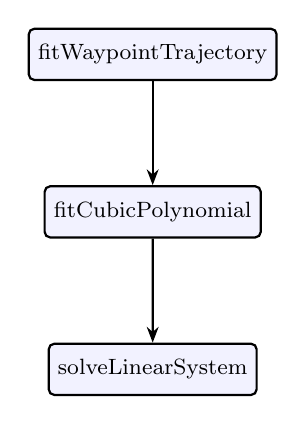
\begin{tikzpicture}[
  level 1/.style={sibling distance=5cm, level distance=2.0cm},
  level 2/.style={sibling distance=3.5cm, level distance=2.0cm},
  every node/.style={rectangle, draw, rounded corners=2pt, thick,
    minimum height=0.65cm, text centered, font=\footnotesize,
    fill=blue!5},
  edge from parent/.style={draw, -{Stealth[length=2mm]}, thick}
]

\node {fitWaypointTrajectory}
  child { node {fitCubicPolynomial}
    child { node {solveLinearSystem} }
  };

\end{tikzpicture}
\end{center}

% ============================================================
%  1.7.1 下级函数需求
% ============================================================
\subsubsection{fitCubicPolynomial~---~三次多项式拟合}

\begin{itemize}
  \item \textbf{功能}：对数据点进行三次多项式最小二乘拟合。
  \item \textbf{输入}：\texttt{xData[]}、\texttt{yData[]}（double 数组）、\texttt{numPoints}（int）。
  \item \textbf{输出}：\texttt{PolynomialCoeffs}（4 个系数 $c_0, c_1, c_2, c_3$）。
  \item \textbf{算法}：构造 Vandermonde 矩阵的法方程 $(\mathbf{A}^{\!\top}\!\mathbf{A})\mathbf{c} = \mathbf{A}^{\!\top}\!\mathbf{y}$，调用 \texttt{solveLinearSystem} 高斯消元求解。
  \item \textbf{异常处理}：线性方程组奇异时返回零系数。
\end{itemize}

% ============================================================
%  1.8 数据结构定义
% ============================================================
\subsection{数据结构定义}

以下数据结构定义于 \texttt{waypointFollowTypes.hpp}，命名空间 \texttt{waypoint\_follow}。

\subsubsection{Waypoint~---~二维路点坐标}
\begin{longtable}{|L{3.5cm}|C{2cm}|L{9.5cm}|}
\hline
\textbf{成员} & \textbf{类型} & \textbf{说明} \\
\hline
\texttt{x} & double & 纵向坐标 (m)，自车坐标系前方为正 \\
\hline
\texttt{y} & double & 横向坐标 (m)，自车坐标系左方为正 \\
\hline
\end{longtable}

\subsubsection{PolynomialCoeffs~---~三次多项式系数}
\begin{longtable}{|L{3.5cm}|C{2cm}|L{9.5cm}|}
\hline
\textbf{成员} & \textbf{类型} & \textbf{说明} \\
\hline
\texttt{c[4]} & double[4] & $y = c_0 + c_1 x + c_2 x^2 + c_3 x^3$ \\
\hline
\end{longtable}

\subsubsection{FittedTrajectory~---~拟合参考轨迹}
\begin{longtable}{|L{3.5cm}|C{2cm}|L{9.5cm}|}
\hline
\textbf{成员} & \textbf{类型} & \textbf{说明} \\
\hline
\texttt{poly} & PolynomialCoeffs & 归一化坐标系下的多项式系数 \\
\hline
\texttt{xOffset} & double & X坐标归一化偏移量 (m) \\
\hline
\texttt{xScale} & double & X坐标归一化缩放因子 (m) \\
\hline
\texttt{refSpeed} & double & 路点推算的参考车速 (m/s) \\
\hline
\texttt{valid} & bool & 轨迹拟合是否有效 \\
\hline
\end{longtable}

% ============================================================
%  1.9 测试用例
% ============================================================
\subsection{测试用例}

\subsubsection{正常测试用例}

{\small
\begin{longtable}{|C{0.6cm}|L{2.2cm}|L{4.8cm}|L{4.0cm}|L{3.5cm}|}
\hline
\textbf{编号} & \textbf{场景} & \textbf{输入} & \textbf{预期输出} & \textbf{验证准则} \\
\hline
\endfirsthead
\hline
\textbf{编号} & \textbf{场景} & \textbf{输入} & \textbf{预期输出} & \textbf{验证准则} \\
\hline
\endhead
N-1 &
直线路点 &
$N{=}6$, $v_e{=}20$, 路点沿 $y{=}0$ 均匀分布, $x_i{=}5i$ &
$c_0{\approx}0$, $c_1{\approx}0$, valid=true &
$|c_2|{<}0.01$, $|c_3|{<}0.01$ \\
\hline
N-2 &
圆弧路点 &
$N{=}6$, $v_e{=}15$, 路点沿 $R{=}100$\,m 圆弧 &
$c_2 \neq 0$, valid=true &
$v_{\text{ref}} \approx 15$\,m/s \\
\hline
N-3 &
S形轨迹路点 &
$N{=}6$, $v_e{=}18$, 路点构成S形 &
$c_3 \neq 0$, valid=true &
拟合有效, $v_{\text{ref}} > 0$ \\
\hline
N-4 &
密集近距路点 &
$N{=}6$, $v_e{=}5$, 路点 $x_i \in [0.5, 3.0]$\,m &
valid=true, $v_{\text{ref}} > 0$ &
$\Delta x \geq 0.5$\,m, 拟合有效 \\
\hline
N-5 &
高速远距路点 &
$N{=}6$, $v_e{=}30$, $x_i$ 达 90\,m &
valid=true, $v_{\text{ref}} \approx 30$ &
归一化后系数数值合理 \\
\hline
\end{longtable}
}

\vspace{6pt}
{\small
\begin{longtable}{|L{2.5cm}|L{13cm}|}
\hline
\multicolumn{2}{|c|}{\textbf{正常测试用例符号说明}} \\
\hline
\textbf{符号} & \textbf{含义} \\
\hline
$N$ & 路点数量 numWaypoints \\
\hline
$v_e$ & 自车车速 egoSpeed (m/s) \\
\hline
$c_0, c_1, c_2, c_3$ & 拟合多项式系数 poly.c[0..3] \\
\hline
$v_{\text{ref}}$ & 输出参考车速 refSpeed (m/s) \\
\hline
$\Delta x$ & X坐标范围 $x_{\max} - x_{\min}$ (m) \\
\hline
$R$ & 圆弧半径 (m) \\
\hline
\end{longtable}
}

\subsubsection{异常测试用例}

{\small
\begin{longtable}{|C{0.6cm}|L{2.0cm}|L{4.5cm}|L{4.2cm}|L{3.8cm}|}
\hline
\textbf{编号} & \textbf{场景} & \textbf{输入} & \textbf{预期输出/行为} & \textbf{验证准则} \\
\hline
\endfirsthead
\hline
\textbf{编号} & \textbf{场景} & \textbf{输入} & \textbf{预期输出/行为} & \textbf{验证准则} \\
\hline
\endhead
A-1 &
路点全重合 &
6 个路点坐标全为 $(0,0)$ &
valid=false, $v_{\text{ref}}{=}v_e$ &
$\Delta x{=}0 < 0.5$ \\
\hline
A-2 &
X跨度过小 &
所有路点 $x \in [0, 0.3]$\,m &
valid=false &
$\Delta x < 0.5$\,m \\
\hline
A-3 &
NaN 路点X坐标 &
\texttt{waypoints[0].x = NaN} &
不崩溃; 拟合可能无效 &
函数正常返回 \\
\hline
A-4 &
NaN 路点Y坐标 &
\texttt{waypoints[3].y = NaN} &
不崩溃; 系数可能含NaN &
函数正常返回 \\
\hline
A-5 &
Infinity X坐标 &
\texttt{waypoints[0].x} $= +\infty$ &
$\Delta x{=}\infty$; 归一化异常 &
函数正常返回, 不崩溃 \\
\hline
A-6 &
Infinity Y坐标 &
\texttt{waypoints[2].y} $= +\infty$ &
法方程可能奇异 &
函数正常返回 \\
\hline
A-7 &
零速输入 &
$v_e{=}0$, 路点正常 &
valid=true, $v_{\text{ref}} > 0$ &
$v_{\text{ref}}$ 由路点间距算出 \\
\hline
A-8 &
负速度输入 &
$v_e{=}{-}10$\,m/s &
拟合正常, $v_{\text{ref}}$ 正常 &
$v_e$ 仅在拟合无效时使用 \\
\hline
A-9 &
极端曲率路点 &
路点 $y$ 值高达 $\pm 50$\,m &
valid=true, 系数很大 &
函数返回, 系数有限 \\
\hline
A-10 &
共线退化路点 &
6个路点共线 $y{=}0.5x$ &
$c_1 \neq 0$, $c_2{\approx}0$, $c_3{\approx}0$ &
线性退化，高阶系数近零 \\
\hline
\end{longtable}
}

\vspace{6pt}
{\small
\begin{longtable}{|L{2.5cm}|L{13cm}|}
\hline
\multicolumn{2}{|c|}{\textbf{异常测试用例符号说明}} \\
\hline
\textbf{符号} & \textbf{含义} \\
\hline
$v_e$ & 自车车速 egoSpeed (m/s) \\
\hline
$\Delta x$ & X坐标范围 $x_{\max} - x_{\min}$ (m) \\
\hline
$v_{\text{ref}}$ & 输出参考车速 refSpeed (m/s) \\
\hline
$c_0, c_1, c_2, c_3$ & 拟合多项式系数 poly.c[0..3] \\
\hline
NaN & IEEE 754 非数值 (Not a Number) \\
\hline
$+\infty$ & IEEE 754 正无穷大 \\
\hline
\end{longtable}
}

\end{document}
